% !TEX root = main.tex

\section{Analysis}
\label{sec:analysis}
The following analysis will be presented in two parts, one which will be before filtering with time domain response of the two signals and then the frequency analysis of these with poles and zeroes. Next an appropriate filter will be applied and the two signals will again be analysed as previously explained.

\subsection{Before filtering}

\subsubsection{Time domain analysis}

First a formal analysis of the man and the woman's voice saying "Hej Lasse" in the time domain. In \cref{fig:time_man} the signal for the man can be seen, with the time in seconds on the x-axis and the magnitude on the y-axis and similarily the womans signal is shown in \cref{fig:time_woman}.

\begin{figure}[h]
	\centering
	\begin{subfigure}{0.45\textwidth}
		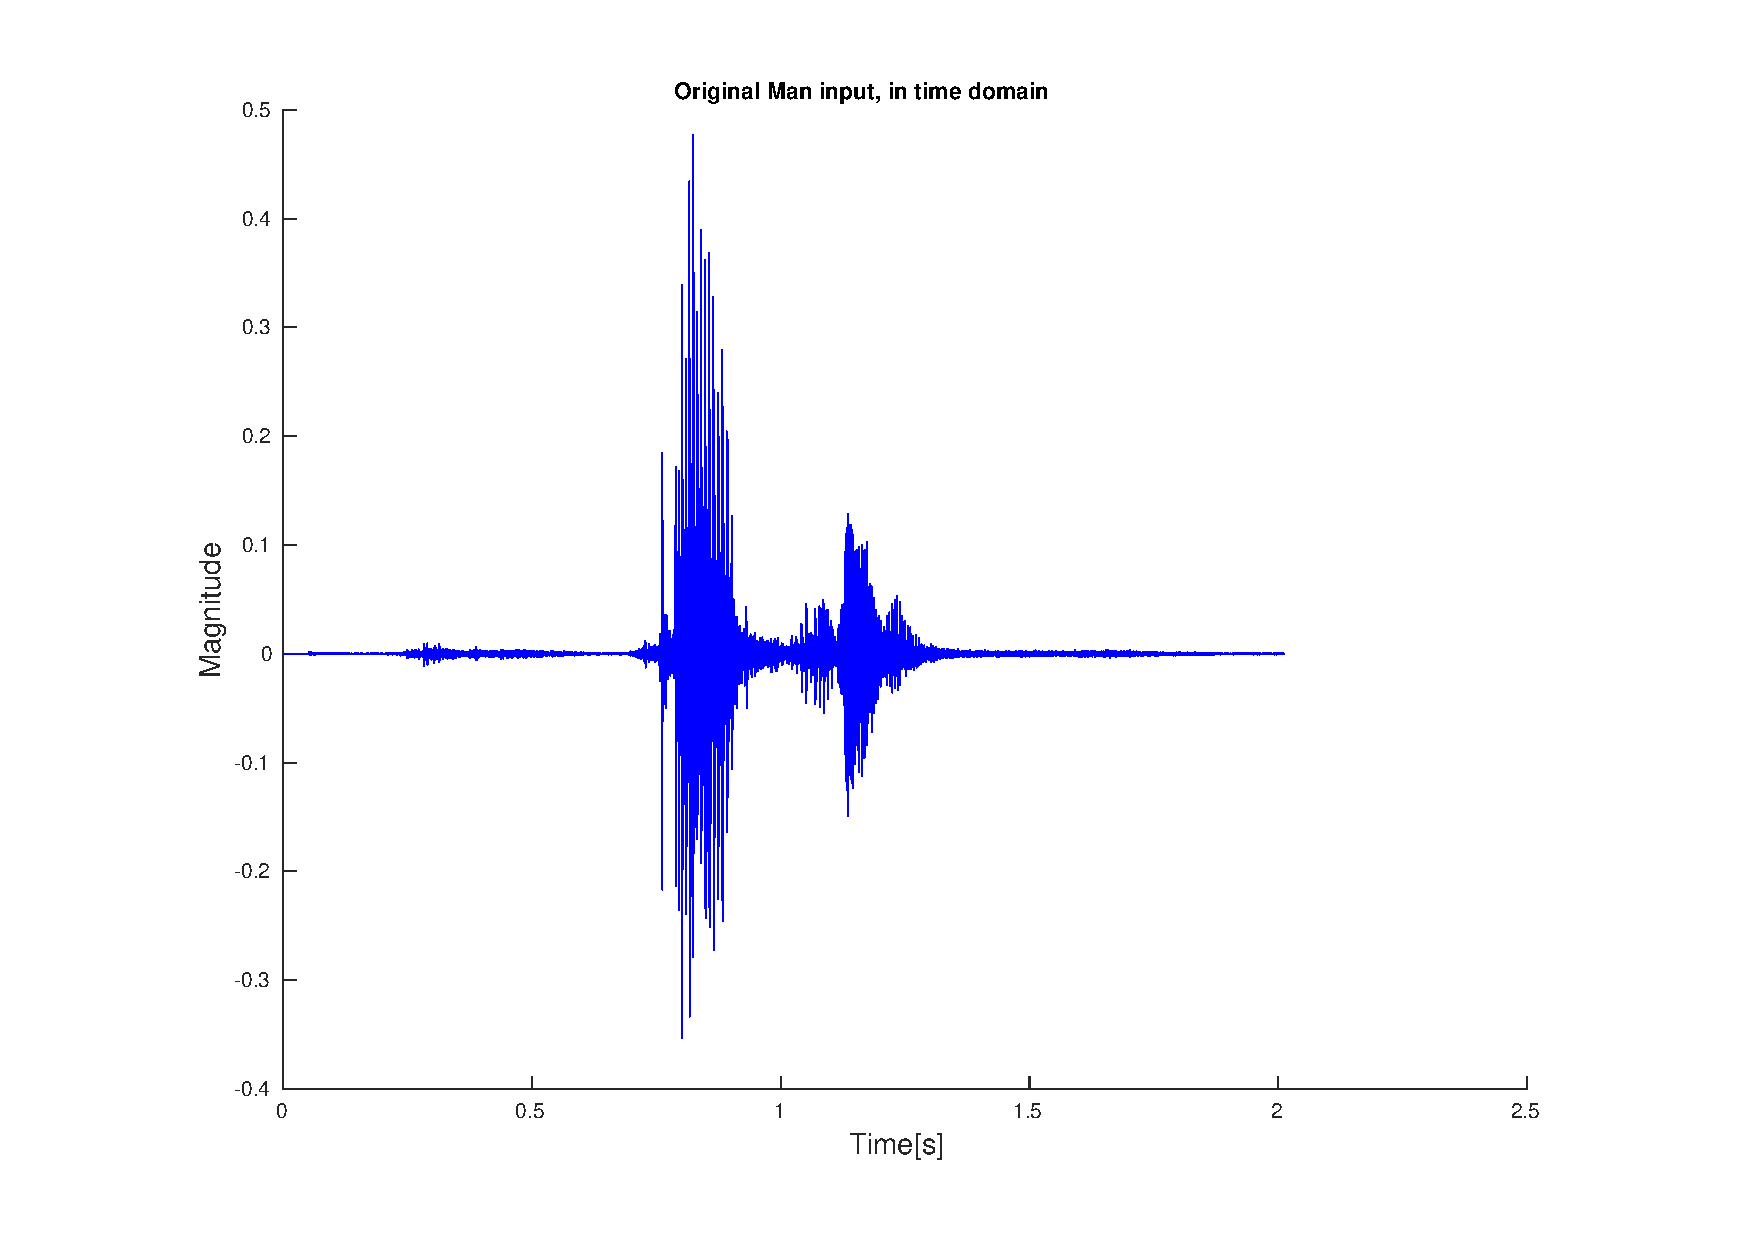
\includegraphics[width=\textwidth]{OrgTid_Man.pdf}
		\caption{The time domain signal of the man.}
		\label{fig:time_man}
	\end{subfigure}
	\quad
	\begin{subfigure}{0.45\textwidth}
		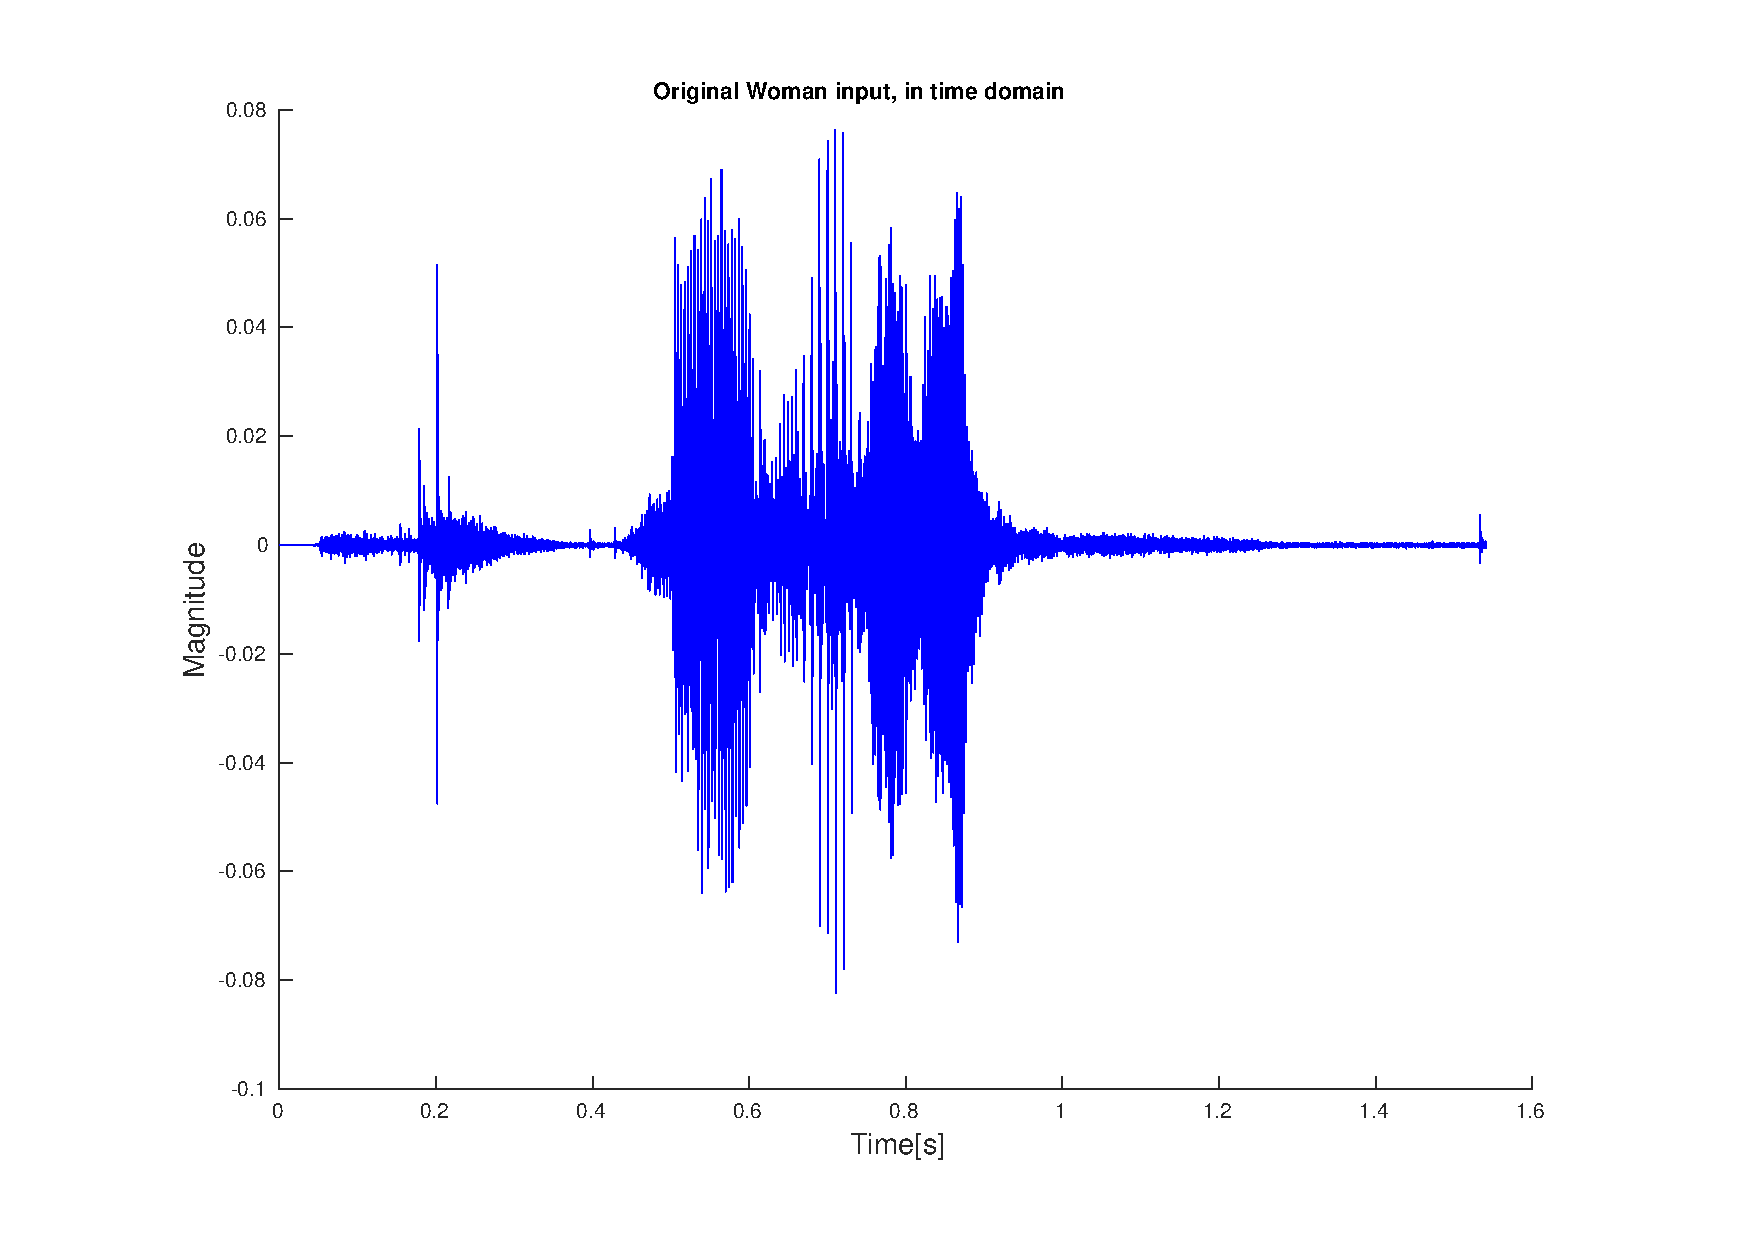
\includegraphics[width=\textwidth]{OrgTid_Woman.pdf}
		\caption{The time domain signal of the woman.}
		\label{fig:time_woman}
	\end{subfigure}
	\caption{The time samples of a man and a woman saying "Hej Lasse".}
	\label{fig:time_WoMan}
\end{figure}

\subsubsection{Fourier transform with FFT}

The fourier transform will show the characteristics of the male and female voice. In \cref{fig:WoManFFT} the fourier transform based of the two previous signals seen in \cref{fig:time_WoMan} - in red the male signal and in blue the female signal. It is clear to see that the primary part of the voice of the male is located at lower frequencies than the voice of the woman.

\begin{figure}[h]
	\centering
	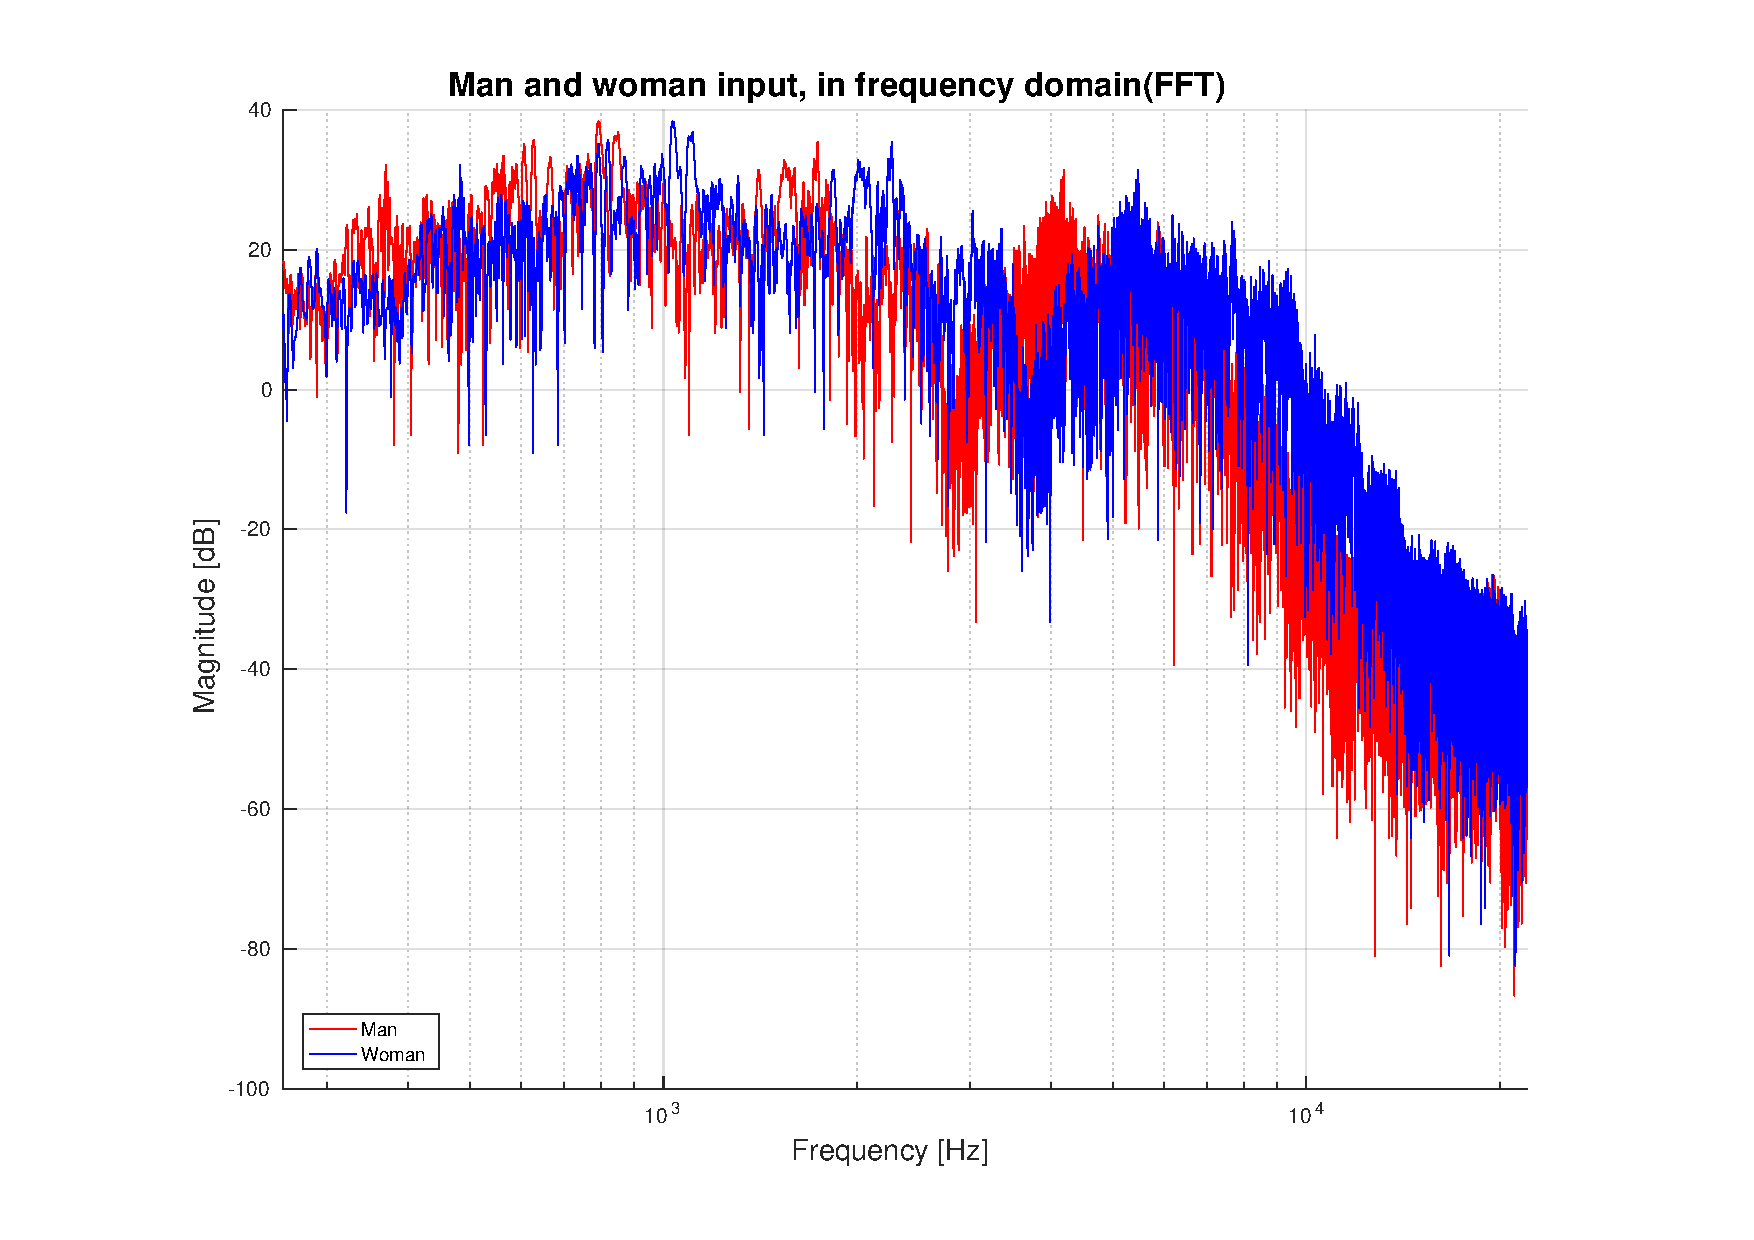
\includegraphics[width=\textwidth]{OrgFreq_WoMan.pdf}
	\caption{The frequency analysis of the man and woman.}
	\label{fig:WoManFFT}
\end{figure}

\subsection{Filtering}

\subsubsection{Highpass filter}
Next up is filtering the signal, which will be done with a highpass filter. From \cref{fig:WoManFFT} a cutoff estimation of \SI{3500}{\hertz} for the female voice and \SI{2800}{\hertz} for the male voice has been chosen. These two cutoff frequencies will be switched for the two signals to see which effect this will have on the signals.

The highpass filter is implemented as a function in matlab and can be seen in the following code example:

\begin{minted}{matlab}
function [figfreq, figHz] = HP(cutFreq, Fs, y, figOrgFreq, figfreqz)
N = length(y);
frequency_samples = [0:Fs/N:(Fs-(Fs/N))];
HighPass = cutFreq/(Fs/2);
HiPass = fir1(70,HighPass,'high');
figfreq = figure(figfreqz);
hold off
title('Filter characteristics');
hold on
freqz(HiPass,1);

% save and visualise 
tic
yHP = filter(HiPass,1,y);
toc
name = ['HP_', num2str(cutFreq), '_Hz.flac'];
audiowrite(name, yHP, Fs);
YHP = fft(yHP);
YdBHP = 20*log10(abs(YHP));

% Plot of discrete fourier transform
figHz = figure(figOrgFreq);
hold off
title(['Original and HP(512 Hz)', ' in frequency domain(FFT)']);
hold on
semilogx(frequency_samples(1:N/2), YdBHP(1:N/2), 'b');
legend({'original', 'highpass'}, 'FontSize', 16);
legend('Location','best');
end
\end{minted}

Notice that the filtered signal is stored as a .flac file, which also will be displayed. The filtered signal can be seen in \cref{fig:HPMAle} for the male and female in \cref{fig:HPFemale}. The filtered signals are somewhat disappointing to listen to, because it simply sounds like \fixme{Like what? hvorfor konklusion her?}

\begin{figure}[h]
	\centering
	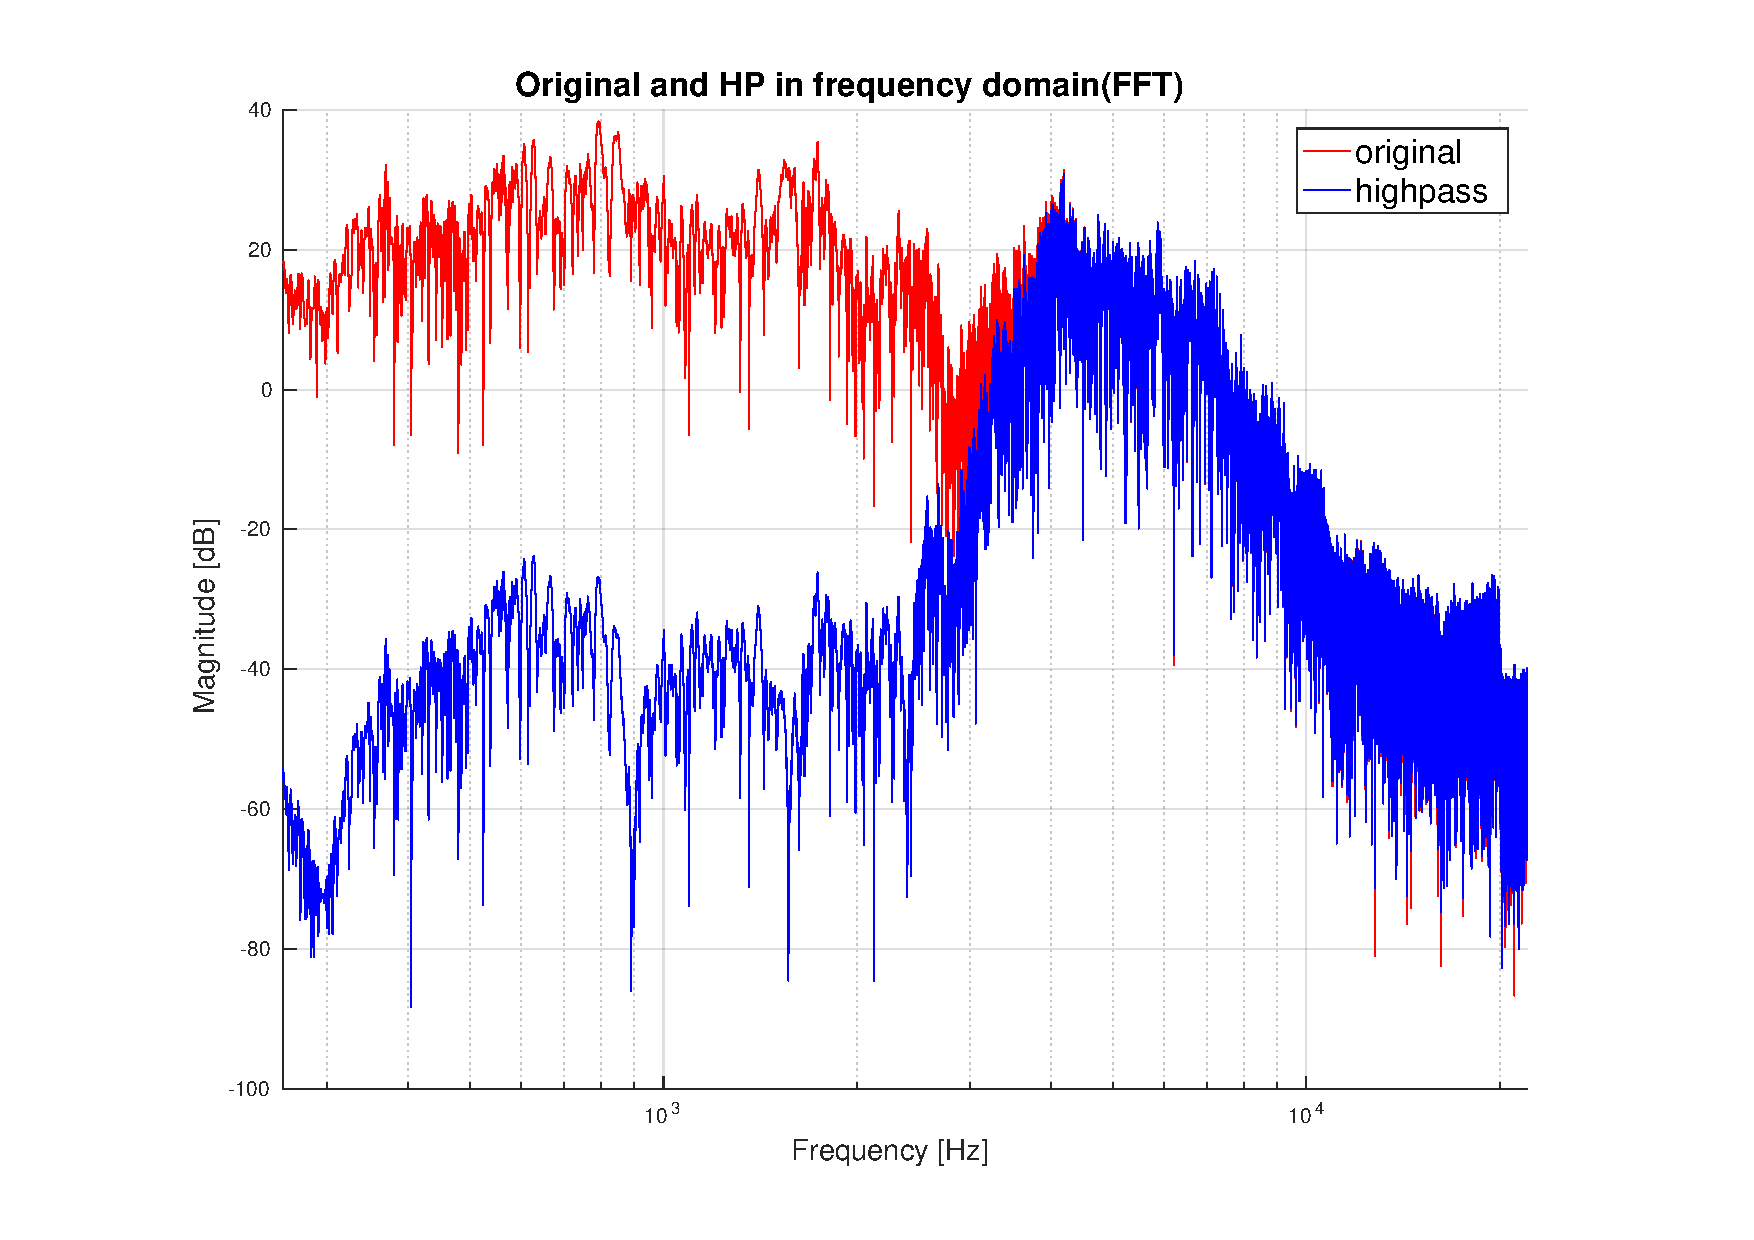
\includegraphics[width=\textwidth]{HPnormFreq_Man.pdf}
	\caption{The highpass filtered signal of the male input.}
	\label{fig:HPMAle}
\end{figure}

\begin{figure}[h]
	\centering
	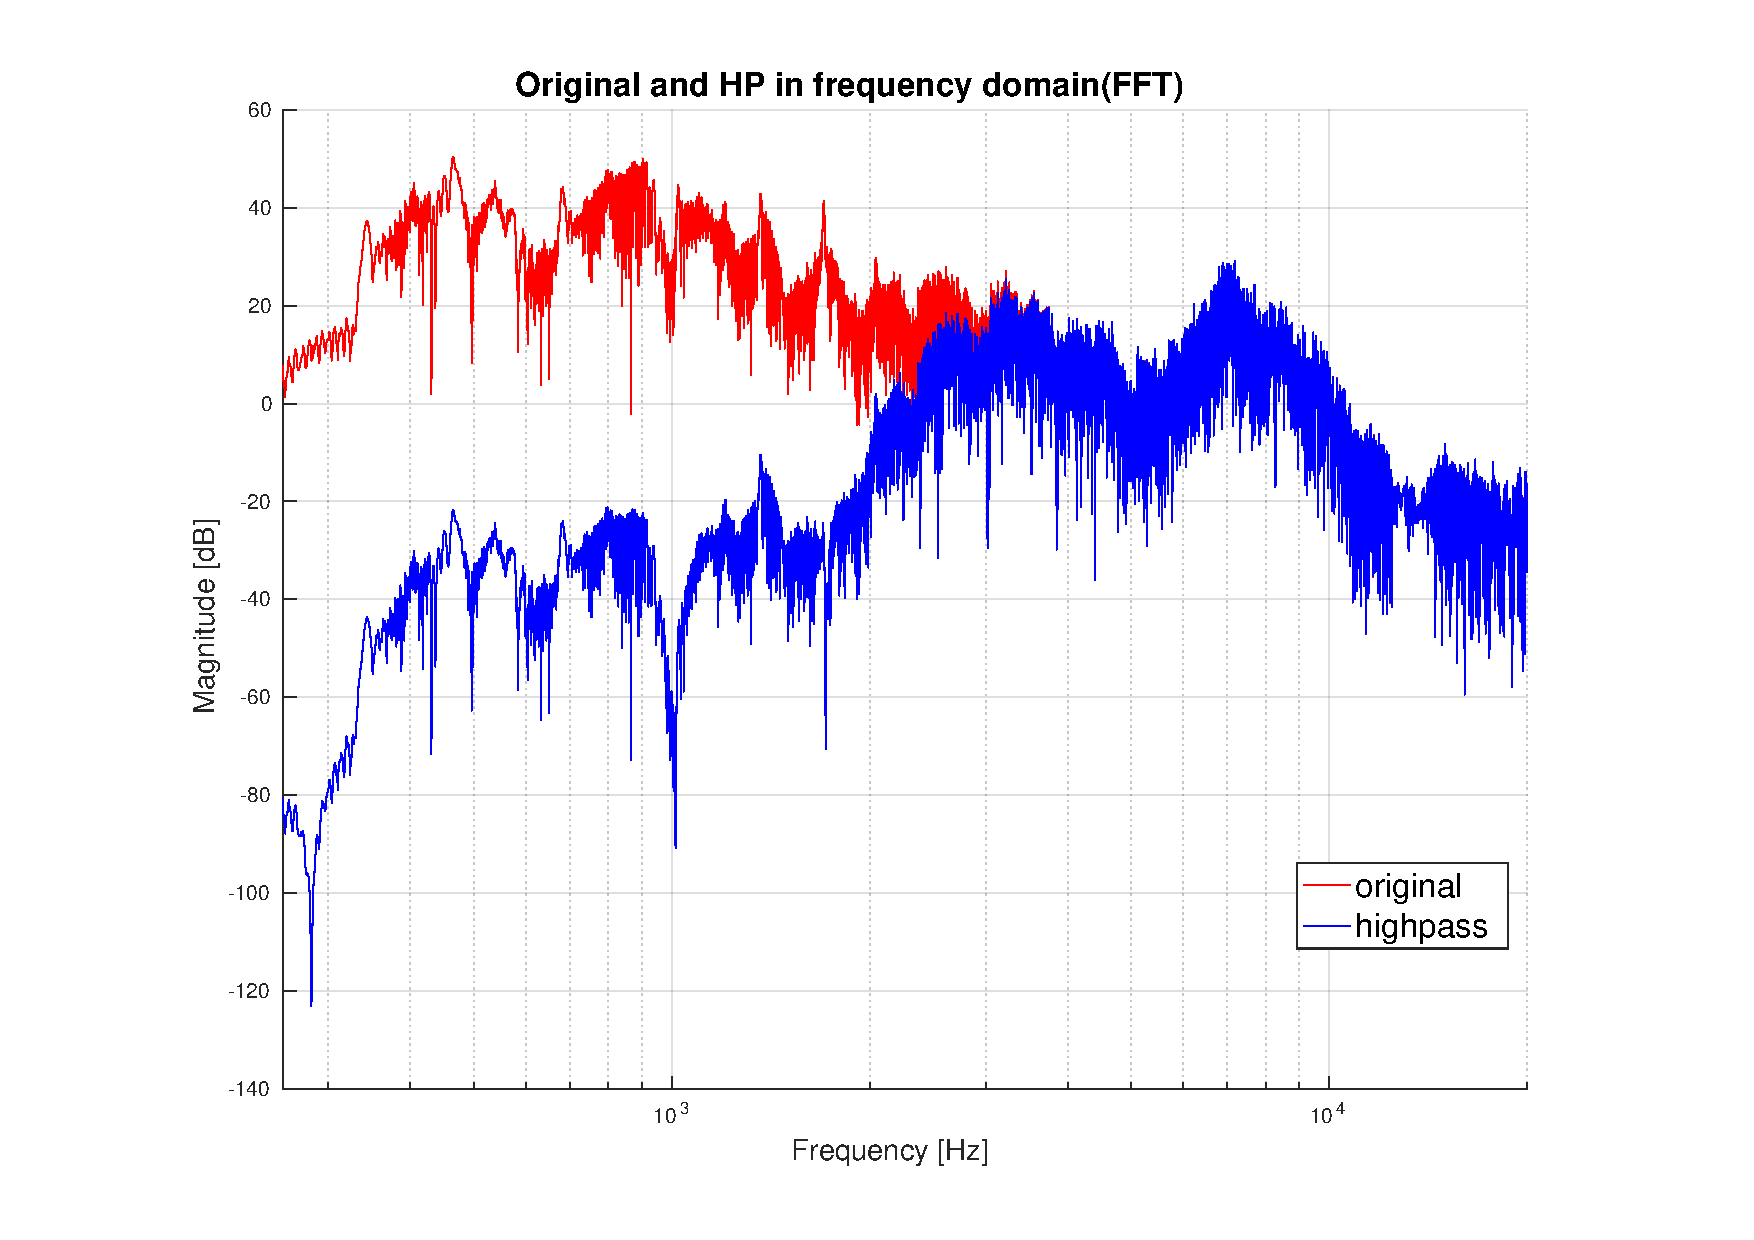
\includegraphics[width=\textwidth]{HPnormFreq_Woman.pdf}
	\caption{The highpass filtered signal of the female input.}
	\label{fig:HPFemale}
\end{figure}

\subsubsection{Bandpass filter (FIR)}
\label{sec:Bandpass}
In the previous section a highpass filter were applied to test which effect it had on the two voices. Now a bandpass filter will be applied with an FIR implementation to the two voices to see which differences there will be. The start of the bandpass filter will again be \SI{2800}{\hertz} for the female signal and \SI{3500}{\hertz} for the male signal, while the cutoffs will be at \SI{8000}{\hertz} for the male signal and \SI{6500}{\hertz} for the female signal. The male filtered signal can be seen in \cref{fig:maleBP} and the female can be seen in \cref{fig:femaleBP}

The code for the bandpass filter is once again implemented in a function and the implementation is as follows:

\begin{minted}{matlab}
function [figW, figHz] = BP(freqRange, Fs, y, figOrgFreq)
N = length(y);
frequency_samples = [0:Fs/N:(Fs-(Fs/N))];
BandPass = freqRange/(Fs/2)
BPass = fir1(100,BandPass,'bandpass');%, kaiser(51,0.5));
figW = figure;
hold on
title('Filter characteristics');
freqz(BPass,1);

% Gem og visualiser frekvensændringen
tic
yBP = filter(BPass,1,y);
toc
name = ['BP_', num2str(freqRange(1)), '_Hz_to_', num2str(freqRange(2)), '_Hz.mp4'];
%audiowrite(name, yBP, Fs);
YBP = fft(yBP);
YdBBP= 20*log10(abs(YBP));

% Plot of discrete fourier transform
figHz = figure(figOrgFreq);
hold off
title({['Original and Bandpass'], [num2str(freqRange(1)), ' Hz to ',...
	num2str(freqRange(2)), ' Hz in frequency domain(FFT)']});
hold on
semilogx(frequency_samples(1:N/2), YdBBP(1:N/2), 'b');
legend({'original', 'bandpass'}, 'FontSize', 16);
legend('Location','best');
end
\end{minted}

\begin{figure}[h]
	\centering
	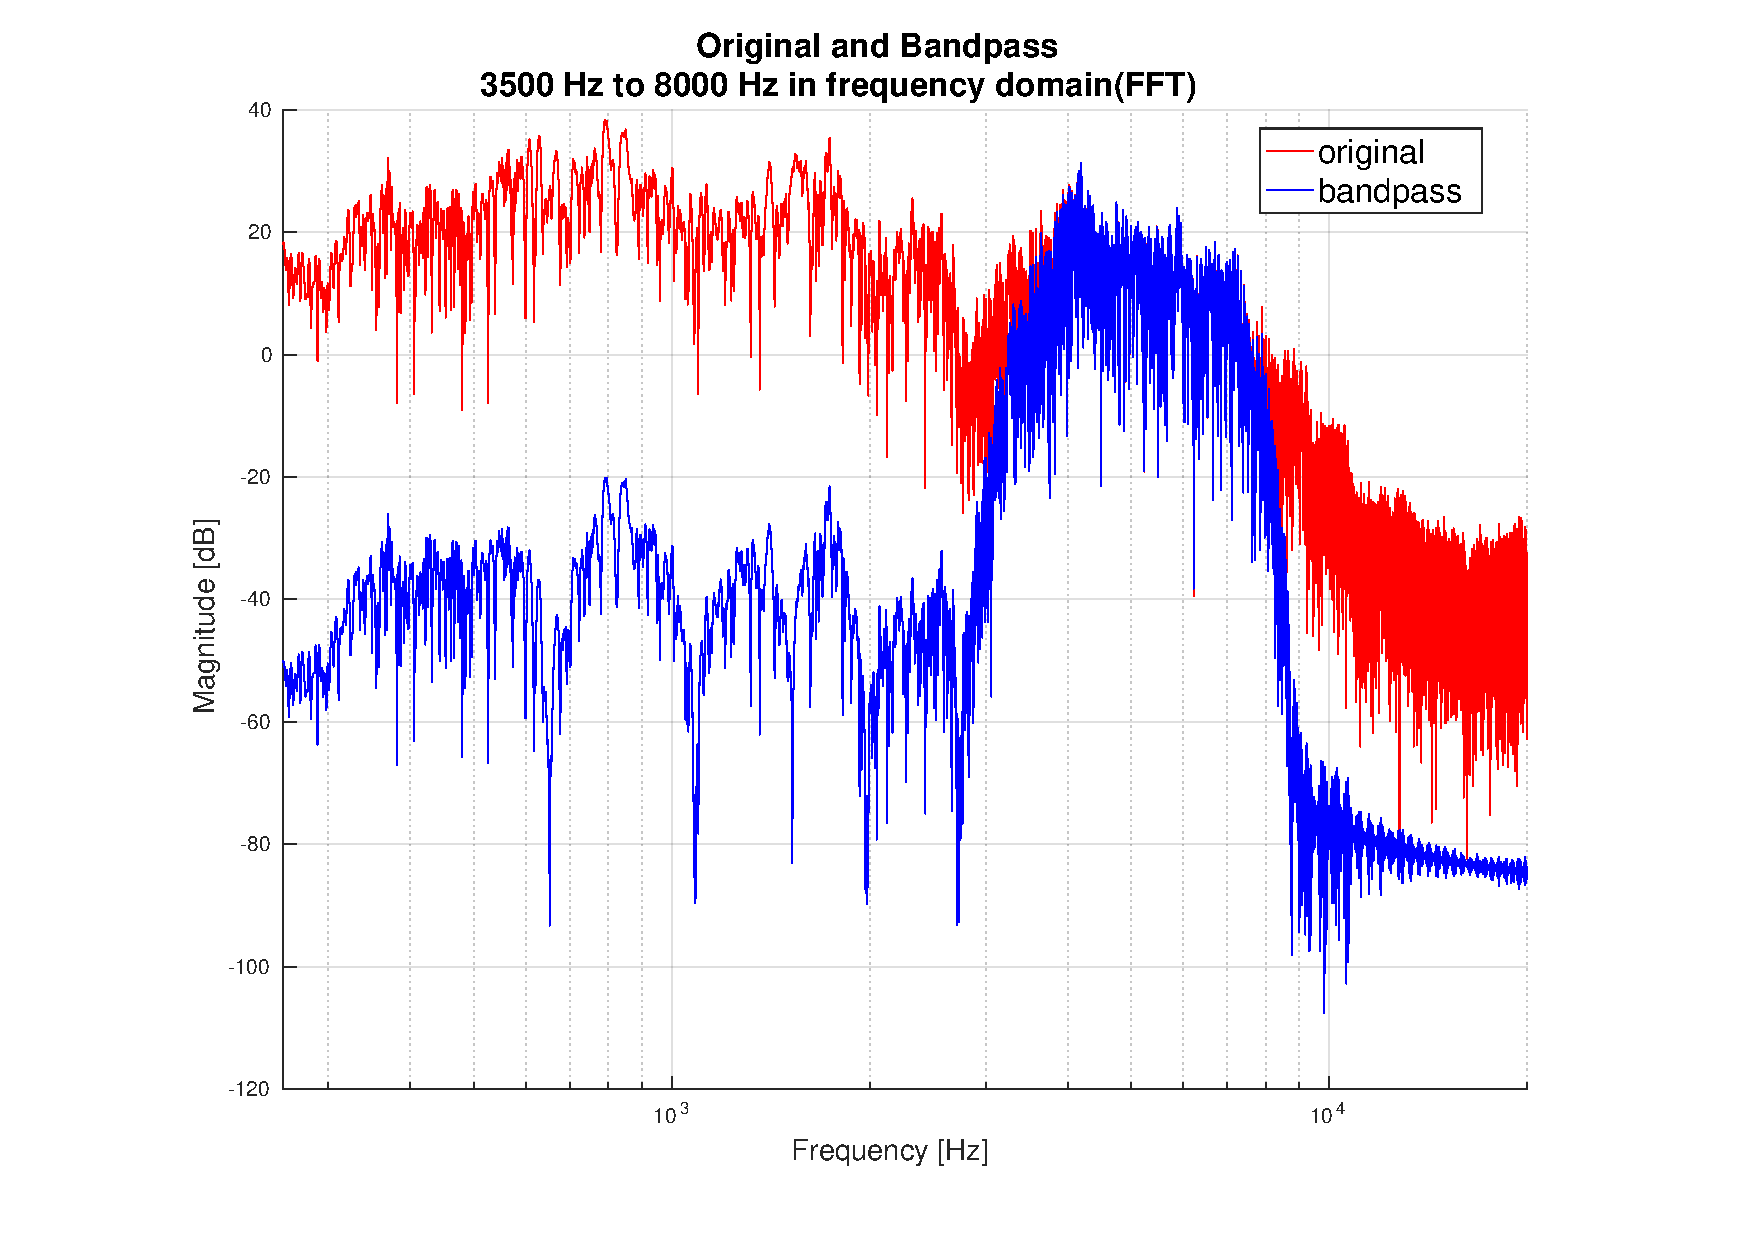
\includegraphics[width=\textwidth]{BP1normFreq_Man.pdf}
	\caption{Bandpass from \SI{3500}{\hertz} to \SI{8000}{\hertz} to the male signal.}
	\label{fig:maleBP}
\end{figure}

\begin{figure}[h]
	\centering
	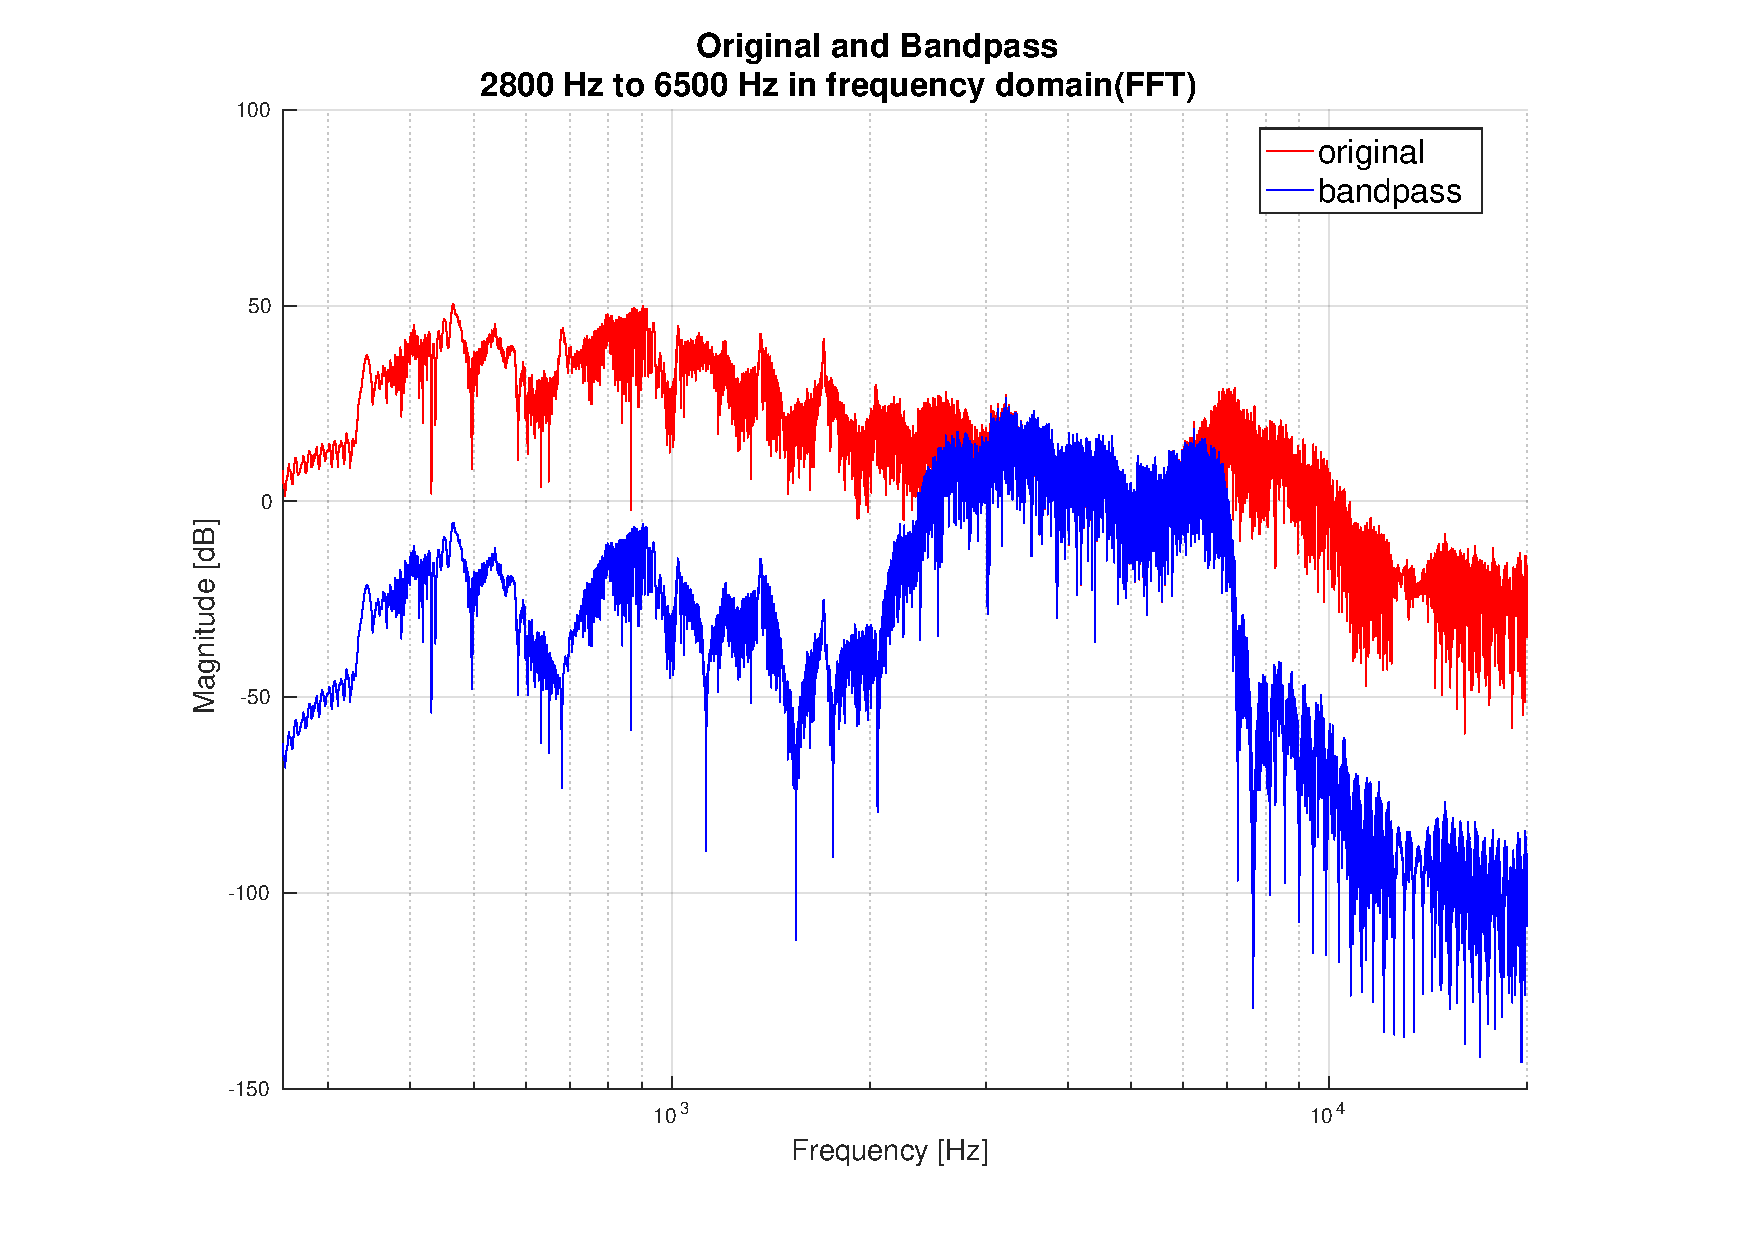
\includegraphics[width=\textwidth]{BP1normFreq_Woman.pdf}
	\caption{Bandpass from \SI{2800}{\hertz} to \SI{6500}{\hertz} to the female signal.}
	\label{fig:femaleBP}
\end{figure}


\subsubsection{Magnitude and phase effect of filtering}
From the section "\nameref{sec:Bandpass}" the frequency response of the filters are analyzed and this data will be analyzed with the function freqz from matlab to tell the magnitude and phase effects of the bandpass filter. In \cref{fig:freqzBP} the effects of phase and magnitude are shown for the female signal and in \cref{fig:freqzBPMale} the male bandpass filter. We expect a phase shift of \ang{-180} per order of the filter - the order is 100 (see code above) hence about \ang{-1800}, which can be seen on female filter \cref{fig:freqzBP} - while the male on \cref{fig:freqzBPMale} have a phase shift of \ang{-2500} which were not expected. The magnitude are damped with about \SI{60}{\decibel} outside of the bandpass filter of both filters, which is clearly seen in the two signals after the bandpass filter (see \cref{fig:maleBP} and \cref{fig:femaleBP})

\begin{figure}[h]
	\centering
	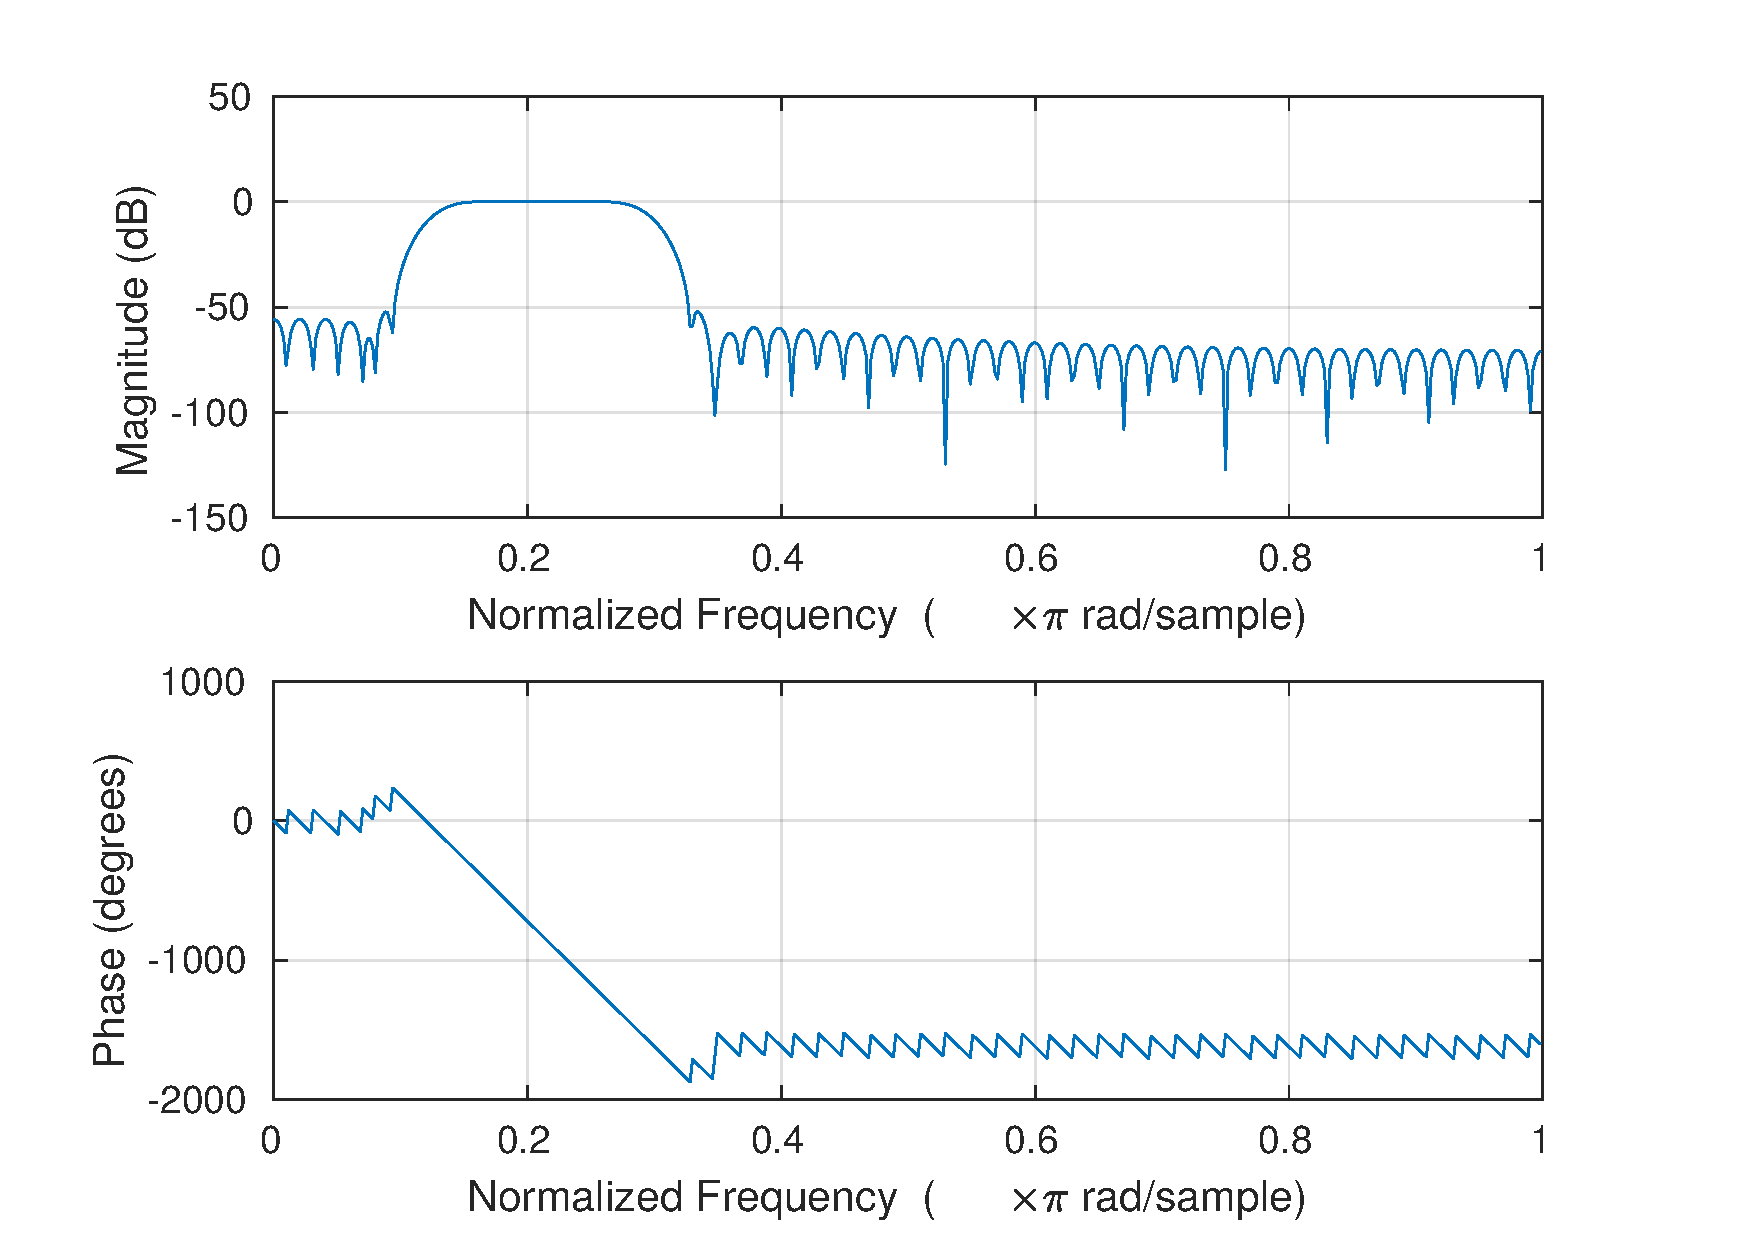
\includegraphics[width=\textwidth]{BandpassFreqz_female-trimmed.pdf}
	\caption{Freqz of the bandpass FIR filter - with the female frequencies}
	\label{fig:freqzBP}
\end{figure}

\begin{figure}[h]
	\centering
	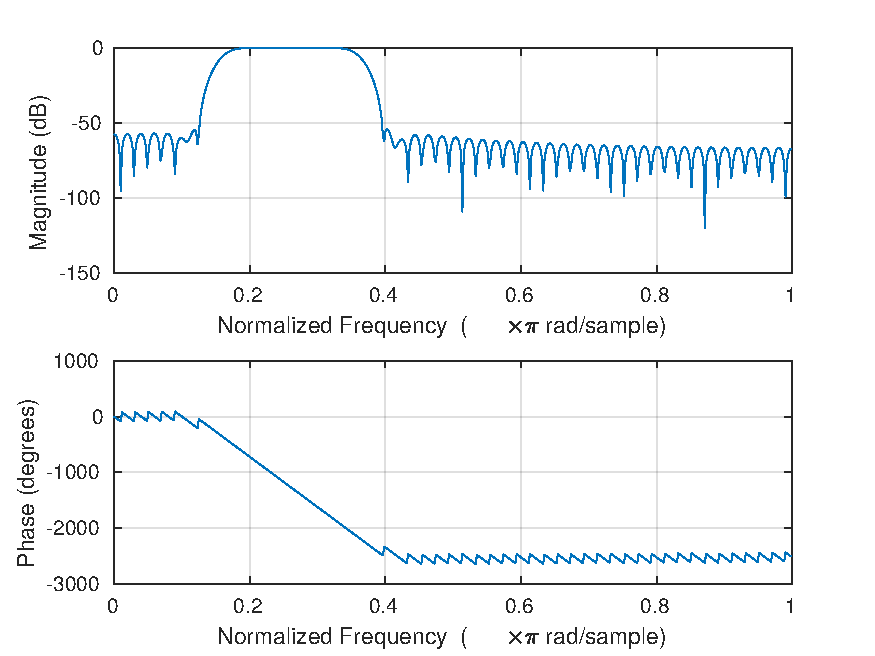
\includegraphics[width=\textwidth]{BandpassFreqz_male-trimmed.pdf}
	\caption{Freqz of the bandpass FIR filter- with the male frequencies}
	\label{fig:freqzBPMale}
\end{figure}

\begin{figure}
	\centering
	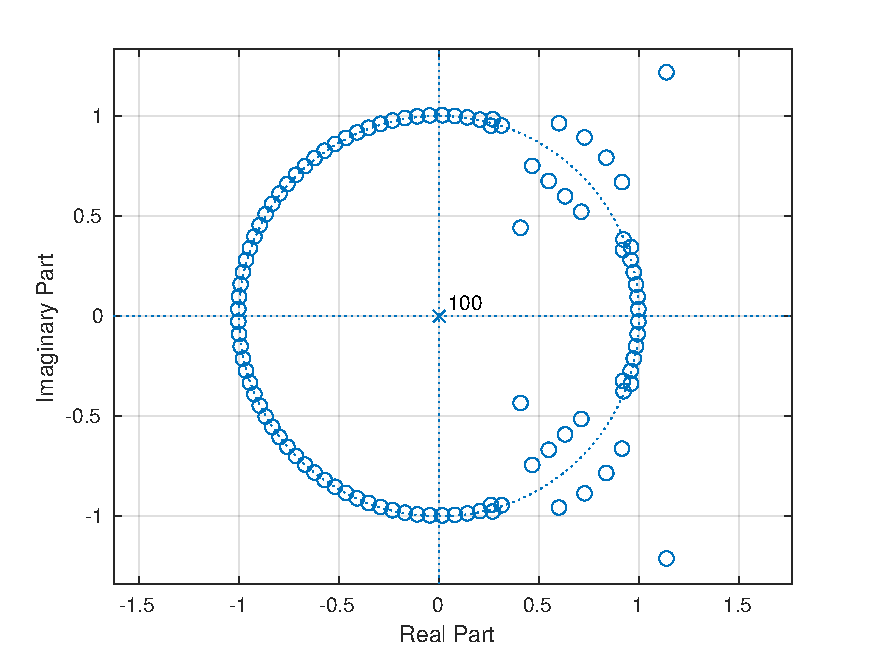
\includegraphics[width=\textwidth]{BP-PZ-trimmed.pdf}
	\caption{The pole-zero plot of the bandpass FIR filter with function zplane}
	\label{fig:BP-zplane}
\end{figure}

In \cref{fig:BP-zplane} the pole-zero plot is shown for the FIR bandpass filter. From this we can see that it is a 100-order filter (100 in the middle, about 0,0) and that it is stable because the poles are located in 0,0 which is within the unitcircle (dotted circle).  

\subsubsection{Bandpass filter (IIR)}
In section "\nameref{sec:Bandpass}" the bandpass filter were made with an FIR filter. In this section we will study the effects of the IIR bandpass filter with the same applied signals and frequencies as seen in section "\nameref{sec:Bandpass}". The filter implementation can be seen in the following code example:

\begin{minted}{matlab}
function [figW, figHz] = IIRBP(freqRange, Fs, y, figOrgFreq)
N = length(y);
frequency_samples = [0:Fs/N:(Fs-(Fs/N))];
BandPass = freqRange/(Fs/2);
[b,a] = butter(5,BandPass,'bandpass');
figW = figure;
hold on
title('Filter characteristics');
freqz(b,a);
figure
zplane(b,a);

% Gem og visualiser frekvensændringen
tic
yBP = filter(b,a,y);
toc
name = ['IIRBP_', num2str(freqRange(1)), '_Hz_to_', num2str(freqRange(2)), '_Hz.mp4'];
%audiowrite(name, yBP, Fs);
YBP = fft(yBP);
YdBBP= 20*log10(abs(YBP));

% Plot of discrete fourier transform
figHz = figure(figOrgFreq);
hold off
title({['Original and Bandpass_{IIR}'], [num2str(freqRange(1)), ' Hz to ',...
	num2str(freqRange(2)), ' Hz in frequency domain(FFT)']});
hold on
semilogx(frequency_samples(1:N/2), YdBBP(1:N/2), 'b');
legend({'original', 'bandpass'}, 'FontSize', 16);
legend('Location','best');
end
\end{minted}

In \cref{fig:IIRBP-male} the male signal applied with the IIR bandpass filter is seen, while in \cref{fig:IIRBP-female} the female is seen. The filtereffects are found with the use of function "freqz" from the matlab library and can be seen in \cref{fig:IIRBPFreqz}. The stability of the filter is evaluated with matlab function zplane, and from \cref{fig:IIRBP-PZ} it is evident that the filter is stable, because all of the poles (x'es) are within the unitcircle. A very noticable difference can be seen between this IIR implementation of the bandpass filters poles and the ones seen in the FIR implementation in \cref{fig:BP-zplane}. 

\begin{figure}[h]
\centering
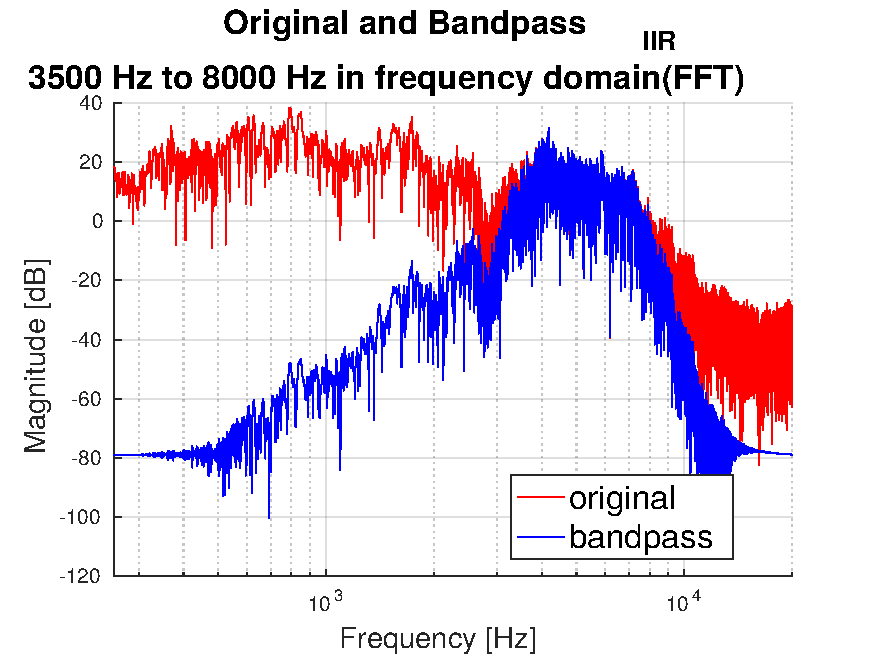
\includegraphics[width=\textwidth]{IIRBP-Male-trimmed.pdf}
\caption{The IIR bandpass filter of the male signal}
\label{fig:IIRBP-male}
\end{figure}

\begin{figure}[h]
\centering
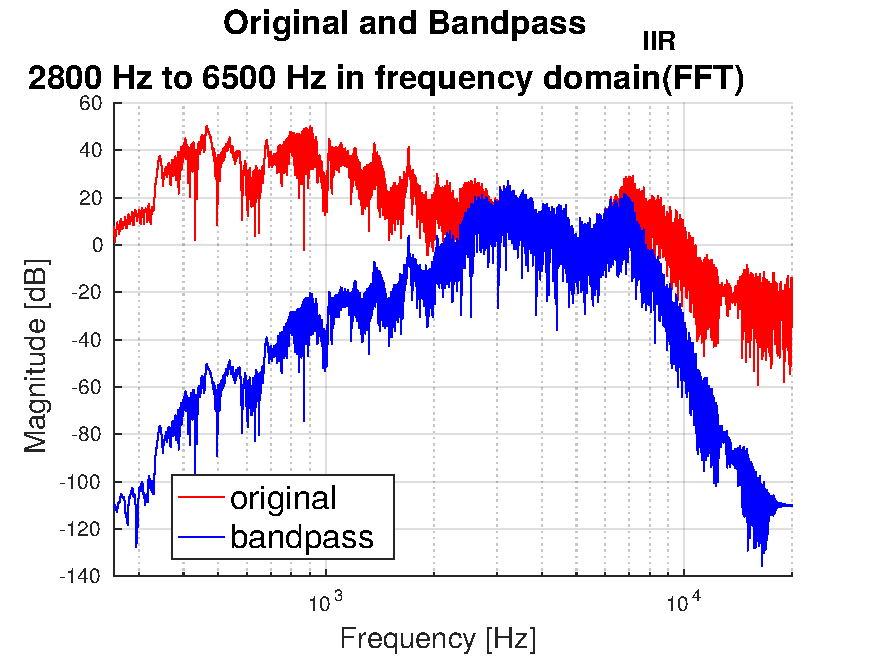
\includegraphics[width=\textwidth]{IIRBP-Female-trimmed.pdf}
\caption{The IIR bandpass filter of the female signal}
\label{fig:IIRBP-female}
\end{figure}

\begin{figure}[h]
\centering
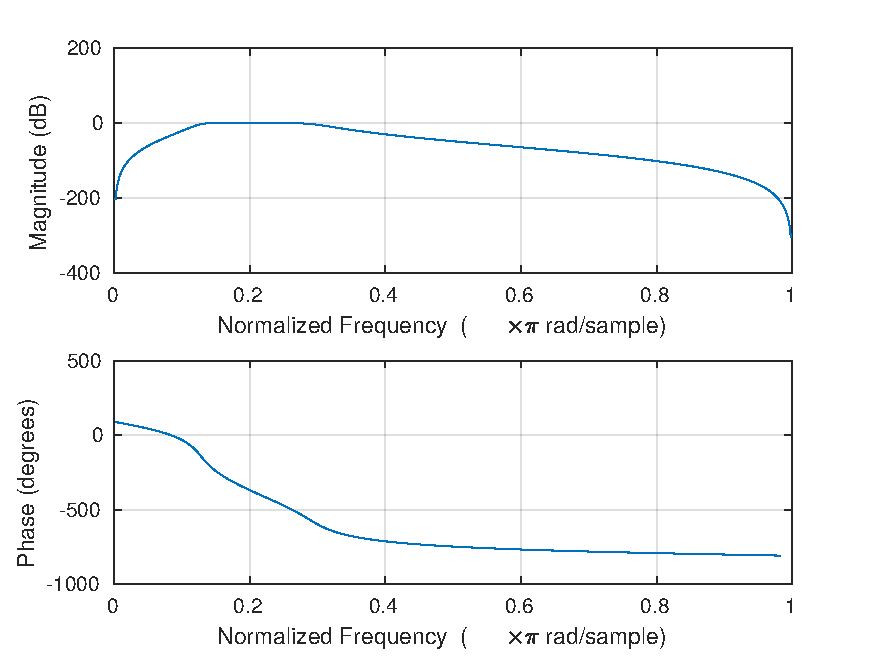
\includegraphics[width=\textwidth]{IIRBPFreqz-trimmed.pdf}
\caption{The Magnitude and phase effects of the IIR bandpass filter}
\label{fig:IIRBPFreqz}
\end{figure}

\begin{figure}[h]
\centering
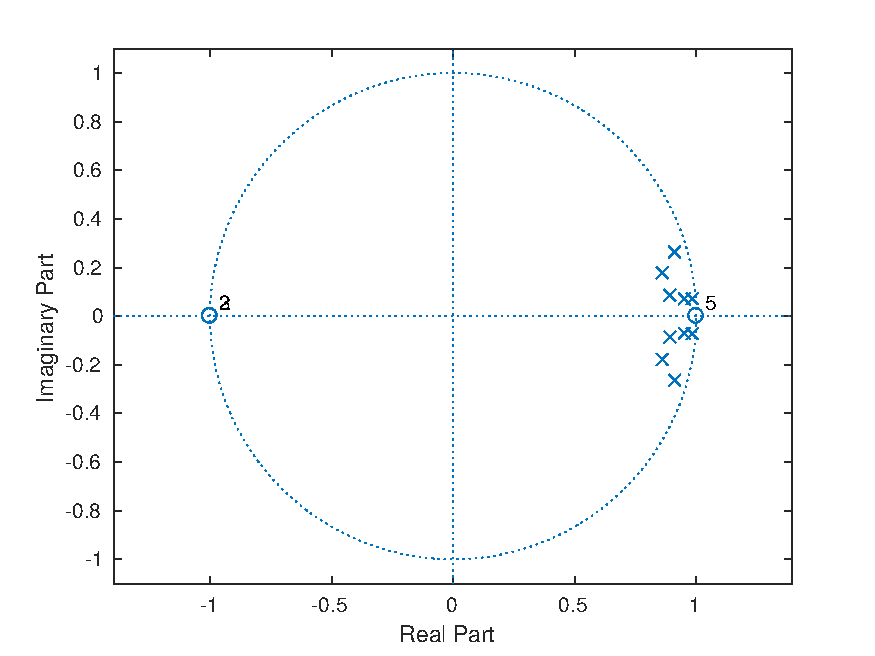
\includegraphics[width=\textwidth]{IIRBP-PZ-trimmed.pdf}
\caption{The pole-zero diagram of the IIR filter}
\label{fig:IIRBP-PZ}
\end{figure}
